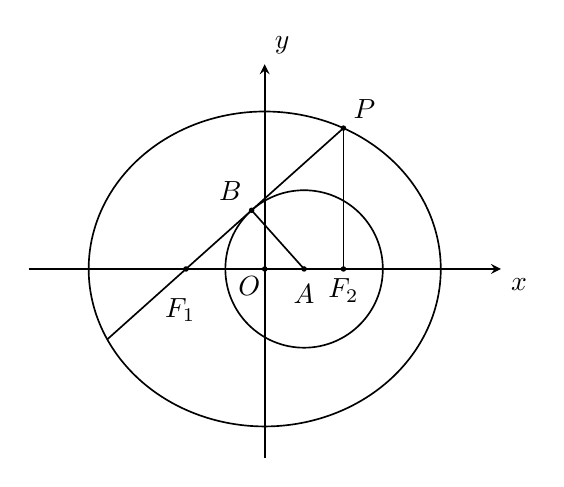
\begin{tikzpicture}[line width=0.6pt, font=\normalsize, >=stealth]
\coordinate (F1) at (-1,0);
\coordinate (F2) at (1,0);
\coordinate (O) at (0,0);
\coordinate (A) at (0.5,0);
\coordinate (P) at (1.0000000000,1.7888543820);
\coordinate (B) at (-0.1666666667,0.7453559925);
\coordinate (Xmin) at (-3,0);
\coordinate (Xmax) at (3,0);
\coordinate (Ymin) at (0,-2.4);
\coordinate (Ymax) at (0,2.6);
% axes
\draw[->] (Xmin) -- (Xmax);
\draw[->] (Ymin) -- (Ymax);
\node[above right] at (Ymax) {$y$};
\node[below right] at (Xmax) {$x$};
% ellipse x^2/5+y^2/4=1 : a=sqrt(5), b=2
\draw plot[domain=0:360, samples=160, smooth] ({sqrt(5)*cos(\x)},{2*sin(\x)});
% circle (x-0.5)^2+y^2=1
\draw (A) circle (1);
% tangent line through F1 and P, extended to left edge of ellipse
\coordinate (Lleft) at (-2.0000000000,-0.8944271910);
\draw (Lleft) -- (P);
% vertical PF2
\draw (P) -- (F2);
% radius AB (center A to tangent point B)
\draw (A) -- (B);
\fill (F1) circle (1pt);
\fill (F2) circle (1pt);
\fill (O) circle (1pt);
\fill (A) circle (1pt);
\fill (B) circle (1pt);
\fill (P) circle (1pt);
\node[below left,xshift=7pt,yshift=-7pt] at (F1) {$F_{1}$};
\node[below] at (F2) {$F_{2}$};
\node[below left,xshift=2pt,yshift=1.0pt] at (O) {$O$};
\node[below, yshift=-2pt] at (A) {$A$};
\node[above left] at (B) {$B$};
\node[above right] at (P) {$P$};
\end{tikzpicture}
